\documentclass[oneside,openany]{ctexbook}
\usepackage{amsmath}
\usepackage{amssymb}
\usepackage{amsfonts}
\usepackage{mathtools}
\usepackage{mathrsfs}
\usepackage[most]{tcolorbox}
\usepackage{float}
\usepackage{geometry}
\usepackage{caption}
\usepackage{graphicx}
\usepackage{indentfirst}
\usepackage{tikz}

\setlength{\parindent}{0pt}

\newtcbtheorem[number within = section]{definition}{定义}{%
  colback = green!5,
  colframe = green!50!black,
  colbacktitle = green!50!black,
  coltitle = white,
  fonttitle = \bfseries,
  fontupper = \itshape,
  attach boxed title to top left = {yshift=-2mm, xshift=5mm},
  separator sign none,
  description delimiters = {(}{)},
  enhanced
}{mydefinition}


\title{抽象代数}
\author{叶超}

\begin{document}

\maketitle

\chapter{群和子群}

\begin{definition}{群}{}
一个群(group)$\langle G,* \rangle$是一个集合G,在一个二元运算*下封闭,且满足以下公理:
\begin{enumerate}
    \item 对于任意$a,b,c\in G$有\\
    $(a*b)*c=a*(b*c)$.  *的结合律(associativity)
    \item G中有一个元素e使得对任意$x\in G$有\\
    $e*x=x*e$.  *的单位元e(identity element)
    \item 对于G中每个元素a,存在元素$a'\in G$有\\
    $a*a'=a'*a=e$.  a的逆元$a'$(inverse)
\end{enumerate}
\end{definition}

\begin{definition}{}{}
设G是一个群,G的阶(order)是G的元素的个数或者基数,记为$|G|$.\\
群元素的阶定义为:
\begin{enumerate}
  \item 若存在最小正整数n,使得\(g^n = e\)(e为群G的单位元),则称g的阶为n,记为\(\text{ord}(g)=n\).
  \item 若不存在这样的正整数n,则称g的阶为无限,记为\(\text{ord}(g)=\infty\).
\end{enumerate}
\end{definition}

\begin{definition}{}{}
如果群G的运算是交换的,那么称它是交换群(阿贝尔群).
\end{definition}

\begin{definition}{}{}
设$\langle G_1,*_1 \rangle$和$\langle G_2,*_2 \rangle$是群,$f:G_1\rightarrow G_2$.如果f满足以下两个条件,就称f是一个群同构(group isomorphism).
\begin{enumerate}
    \item 映射f是即单又满的.
    \item 对于所有$a,b\in G_1,f(a*_1b)=f(a)*_2f(b)$.
\end{enumerate}
其中条件2,称之为同态性质(homomorphism property).
\end{definition}

\begin{table}[h!]
    \centering
    \begin{minipage}[t]{0.45\linewidth}
        \centering
        \small
        \caption{$\mathbb{Z}_4$}
        \begin{tabular}{c|c|c|c|c}
          $+_4$& 0& 1& 2& 3\\
          \hline
          0& 0& 1& 2& 3\\
          \hline
          1& 1& 2& 3& 0\\
          \hline
          2& 2& 3& 0& 1\\
          \hline
          3& 3& 0& 1& 2\\
        \end{tabular}
    \end{minipage}
    \hfill
    \begin{minipage}[t]{0.45\linewidth}
        \centering
        \small
        \caption{克莱因四元群}
        \begin{tabular}{c|c|c|c|c}
          *& e& a& b& c\\
          \hline
          e& e& a& b& c\\
          \hline
          a& a& e& c& b\\
          \hline
          b& b& c& e& a\\
          \hline
          c& c& b& a& e\\
        \end{tabular}
    \end{minipage}
\end{table}

\section{子群}

\begin{definition}{}{}
如果群G的一个非空子集H在G的二元运算下是封闭的,在G的诱导运算下H是一个群,那么称为G的一个子群(subgroup),
用记号$H\leqslant G$或者$G\geqslant H$表示.$H<G$或者$G>H$表示$H\leqslant G$但$H\neq G$
\end{definition}

\begin{definition}{}{}
如果G是一个群,那么由G本身组成的子群是G的非真子群(improper subgroup),其他子群都是真子群(proper subgroup).
子群$\{e\}$和G是G的平凡子群(trivial subgroup),所有其他子群都是非平凡子群(nontrivial subgroup).
\end{definition}

\begin{definition}{}{}
群G的子集H是G的子群当且仅当:
\begin{enumerate}
  \item H在G的二元运算下是封闭的,
  \item G的单位元e在H中;
  \item 对于所有的$a\in H$,也有$a^{-1}\in H$.
\end{enumerate}
\end{definition}

\begin{definition}{}{}
如果$\langle a\rangle=G$,称群G由元素a生成(generate),并称a为G的生成元(generator).
如果G中有一个元素a生成G,称G为循环的(cyclic).
\end{definition}

\section{循环群}

\begin{definition}{}{}
每个循环群都是交换群.
\end{definition}

\begin{definition}{}{}
循环群的子群是循环的.
\end{definition}

\begin{definition}{}{}
加法群$\mathbb{Z}$的全部子群恰好是所有的加法群$n\mathbb{Z}$,$n\in \mathbb{Z}$.
\end{definition}

\begin{definition}{}{}
设G是生成元为a的循环群,如果G是无限阶的,那么G同构于$\langle\mathbb{Z},+\rangle$.\\
如果G的阶为n,则G同构于$\langle\mathbb{Z}_n,+_n\rangle$.
\end{definition}

\begin{definition}{}{}
设G是一个有限循环群,$H\leq G$.那么$|H|$整除$|G|$.也就是说,$|G|$是$|H|$的倍数.
\end{definition}

\chapter{群结构}

\begin{definition}{}{}
设G和$G'$之间有映射$\phi :G\rightarrow G'$.如果同态性质$$\phi (ab)=\phi (a)\phi (b)$$
对所有$a,b\in G$成立,则称映射$\phi$为同态(homomorphism). 
\end{definition}

\begin{definition}{}{}
设$\phi$是群G到群$G'$的同态.
\begin{enumerate}
  \item 如果e是G中的单位元,那么$\phi (e)$是$G'$中的单位元$e'$.
  \item 如果$a\in G$,那么$\phi (a^{-1})=\phi(a)^{-1}$.
  \item 如果H是G的子群,那么$\phi [H]$是$G'$的子群.
  \item 如果$K'$是$G'$的子群,那么$\phi ^{-1}[K']$是G的子群.
\end{enumerate}
也就是说,$\phi$保持单位元、逆元和子群.
\end{definition}

\begin{definition}{}{}
设$\phi :G\rightarrow G'$是群同态.子群$\phi ^{-1}[\{e^{-1}\}]=\{x\in G|\phi (x)=e'\}$称为$\phi$的核(kernel),\\
记为$Ker(\phi)$.
\end{definition}

核的含义是在$\phi$的映射下,原来G中的元素被映射成了$G'$中的单位元,这部分属于G的元素构成的子群,称为核.

\begin{definition}{凯莱定理}{}
每个群与一个置换群同构.
\end{definition}

\section{有限生成交换群}

\begin{definition}{笛卡尔积}{}
集合$B_1,B_2,\cdots ,B_n$的笛卡尔积(Cartesian product)是所有n元有序组$(b_1,b_2,\cdots ,b_n)$的集合,其中$b_i\in B_i,i=1,2,\cdots ,n$.笛卡尔积记为
$$B_1\times B_2\times \cdots \times B_n$$或$$\prod ^n_{i=1}B_i$$
\end{definition}

笛卡尔积的含义是集合$B_1,B_2,\cdots ,B_n$中的元素的全排列构成的集合$B'$.\\
设$b_i\in B_i,i=1,2,\cdots ,n$,则$B'$的元素为$(b_1,b_2,\cdots b_n)$\\
例$\mathbb{Z}_2=\{0,1\}$,$\mathbb{Z}_3=\{0,1,2\}$,则$\mathbb{Z}_2 \times \mathbb{Z}_3=\{(0,0),(0,1),(0,2)(1,0),(1,1),(1,2)\}$.

\begin{definition}{直积}{}
设$G_1,G_2,\cdots ,G_n$为群.对于$\prod ^n_{i=1}G_i$中$(a_1,a_2,\cdots ,a_n)$和$(b_1,b_2,\cdots ,b_n)$,\\
定义$(a_1,a_2,\cdots a_n)(b_1,b_2,\cdots b_n)$为元素$(a_1b_1,a_2b_2,\cdots ,a_nb_n)$.\\
那么$\prod ^n_{i=1}G_i$是一个群,称为$G_i$的直积(direct product).
\end{definition}

直积的含义是$\langle G_1,*_1\rangle,\langle G_2,*_2\rangle,\cdots ,\langle G_n,*_n\rangle$在笛卡尔积下构成群$\langle G',*'\rangle$,\\
设$a_i\in \langle G_i,*_i\rangle,i=1,2,\cdots ,n$,则群$\langle G',*'\rangle$的元素是$(a_1, a_2,\cdots a_n)$.\\
群$\langle G',*'\rangle$的运算由各个群$\langle G_n,*_n\rangle$的运算给出.设$a_i,b_i\in \langle G_i,*_i\rangle,i=1,2,\cdots ,n$,\\则$(a_1, a_2,\cdots a_n)*'(b_1, b_2,\cdots b_n)=(a_1 *_1 b_1, a_2 *_2 b_2,\cdots a_n*_n b_n) \in G'$.

\begin{definition}{}{}
群$\mathbb{Z}_m\times \mathbb{Z}_n$是循环的,并且与$\mathbb{Z}_{mn}$同构,当且仅当m与n互素,即m和n的最大公因子为1.
\end{definition}

\begin{definition}{}{}
设$(r_1,r_2,\cdots ,r_n)\in \prod ^n_{i=1}$.如果$a_i$在$G_i$中有有限阶$r_i$,那么$(a_1,a_2,\cdots ,a_n)$在$\prod ^n_{i=1}$中的阶等于所有$r_i$的最小公倍数.
\end{definition}

\begin{definition}{}{}
每个有限生成交换群G同构于一些循环群的直积,形如$$\mathbb{Z}_{{p_1}^{r_1}}\times \mathbb{Z}_{{p_2}^{r_2}}\times \cdots \times \mathbb{Z}_{{p_n}^{r_n}}\times \mathbb{Z} \times \mathbb{Z} \times \cdots \times \mathbb{Z}$$
其中$p_i$是素数,不一定是不同的,$r_i$是正整数.除了可能的因子重排.直积是唯一的;也就是说,因子$\mathbb{Z}$的数量\textnormal{[G的贝蒂(Betti)数]}是唯一的,素数幂${p_i}^{r_i}$是唯一的.
\end{definition}

\begin{definition}{}{}
每个有限生成交换群同构于一些循环群的直积,形如$$\mathbb{Z}_{d_1}\times \mathbb{Z}_{d_2}\times \mathbb{Z}_{d_3}\times \cdots \times \mathbb{Z}_{d_k}\times \mathbb{Z} \times \mathbb{Z} \times \cdots \times \mathbb{Z}$$
其中每个$d_i\geq 2$是一个整数,$d_i$整除$d_{i+1}$,$1\leq i \leq k-1$.而且这种表示是唯一的.
\end{definition}

例与360阶交换群同构的全部交换群:
\begin{enumerate}
  \item $\mathbb{Z}_2\times \mathbb{Z}_2\times \mathbb{Z}_2\times \mathbb{Z}_3\times \mathbb{Z}_3\times \mathbb{Z}_5$
  \item $\mathbb{Z}_2\times \mathbb{Z}_2\times \mathbb{Z}_2\times \mathbb{Z}_9\times \mathbb{Z}_5$
  \item $\mathbb{Z}_2\times \mathbb{Z}_4\times \mathbb{Z}_3\times \mathbb{Z}_3\times \mathbb{Z}_5$
  \item $\mathbb{Z}_2\times \mathbb{Z}_4\times \mathbb{Z}_9\times \mathbb{Z}_5$
  \item $\mathbb{Z}_8\times \mathbb{Z}_3\times \mathbb{Z}_3\times \mathbb{Z}_5$
  \item $\mathbb{Z}_8\times \mathbb{Z}_9\times \mathbb{Z}_5$
\end{enumerate}

\section{陪集和拉格朗日定理}

\begin{definition}{}{}
设H是群G的子群.$a\in G$,G的子集$aH=\{ah|h\in H\}$称为包含a的H是左陪集(left coset).
同理,G的子集$Ha=\{ha|h\in H\}$称为包含a的H是右陪集(right coset).
\end{definition}

\begin{definition}{}{}
设H是群G的子群.那么对于任何$a\in G$,陪集aH的基数与H的相同.
\end{definition}

\begin{definition}{拉格朗日定理}{}
设H是有限群G的子群,那么H的阶是G的阶的因数.
\end{definition}

\begin{definition}{}{}
素数阶群都是循环的.
\end{definition}

\begin{definition}{}{}
有限群元素的阶整除群的阶.
\end{definition}

\begin{definition}{}{}
设H是群G的子群.G中H的左陪集的数量称为G中H的指数(index),记为$(G:H)$.
\end{definition}

\begin{definition}{}{}
设H和K是G群的子群.$K\leq H\leq G$.假设$(H:K)$和$(G:H)$都是有限的.那么$(G:K)$是有限的,并且$(G:K)=(G:H)(H:K)$.
\end{definition}

\section{左陪集和右陪集}

\begin{definition}{}{}
设$\phi :G\rightarrow G'$是群同态.那么$Ker(\phi)$的左陪集和右陪集是相同的.\\
此外,$a,b\in G$在$Ker(\phi)$的同一个陪集中当且仅当$\phi(a)=\phi(b)$.
\end{definition}

\begin{definition}{}{}
同态$\phi :G\rightarrow G'$是单射当且仅当$Ker(\phi)$是G的平凡子群.
\end{definition}

\chapter{同态和商群}

\begin{definition}{}{}
设H是G的子群.如果对于$g\in G$有$gH=Hg$,称H是G的正规(normal)子群.如果H是G的子群,记为$H\unlhd G$.
\end{definition}

\begin{definition}{}{}
设H是G的正规子群,那么H的陪集$G/H$在二元运算$(aH)(bH)=(ab)H$下构成群.\\
群$G/H$称为G对H的因子群(factor group)或商群(quotient group).
\end{definition}

\begin{definition}{}{}
设H是G的正规子群,那么$\gamma (x)=xH$给出的$\gamma :G\rightarrow G/H$是一个核为H的群同态. 
\end{definition}

\begin{definition}{同态基本定理}{}
设$\phi :G\rightarrow G'$是一个具有核H的群同态.那么$\phi [G]$是一个群,并且由$\mu (gH)=\phi (g)$
给出的$\mu :G/H\rightarrow \phi [G]$是一个群同构.如果$\gamma :G\rightarrow G/H$是由$\gamma (g)=gH$
给出的同态,则对每个$g\in G$有$\phi (g)=\mu \circ \gamma(g)$.
\end{definition}

\begin{figure}
  \centering
  \begin{tikzpicture}[>=latex, thick, font=\small]
    \draw[->](0.2, -0.2)--(6.2, -0.2);
    \draw[->](0.2, -0.3)--(3.2,-3.2);
    \draw[->,dashed](3.5,-3.2)--(6.2, -0.3);
    \node at(0, -0.2){$G$};
    \node at(3.1, 0.1){$\phi$};
    \node at(1.0, -1.8){$\gamma _H$};
    \node at(6.0, -1.8){$\mu$(同构)};
    \node at(3.3, -3.5){$G/H$};
    \node at(6.6, -0.2){$\phi [G]$};
  \end{tikzpicture}
\end{figure}

\section{正规子群与自同构}

\begin{definition}{}{}
以下是群G的子群H为G的正规子群的四个等价条件.
\begin{enumerate}
  \item $ghg^{-1}\in H$对于所有$g\in G$和$h\in H$成立.
  \item $gHg^{-1}=H$对于所有$g\in G$成立.
  \item 存在群同态$\phi :G\rightarrow G'$,使得$Ker(\phi)=H$.
  \item $gH=Hg$对所有$g\in G$成立.
\end{enumerate}
条件2通常视为H是G得到正规子群的定义.
\end{definition}

\begin{definition}{}{}
群G的同构$\phi :G\rightarrow G$称为G的自同构(automorphism).自同构$i_g :G\rightarrow G$对所有$x\in G$
有$i_g(x)=gxg^{-1}$,称为由g生成的G的内自同构(inner automorphism).变换$i_g$在x上的作用称为g对x的共轭(conjugation).
\end{definition}

\section{商群计算和单群}

\begin{definition}{}{}
设$G=H\times K$是群H和K的直积,则$\overline{H}={(h,e)|h\in H}$是G的正规子群.并且$G/\overline{H}$与K自然同构.\\
同样,自然有$G/\overline{K}\cong H$.
\end{definition}

\begin{definition}{}{}
如果G是循环群,N是G的子群,那么$G/N$是循环群.
\end{definition}

\section{单群}

\begin{definition}{}{}
如果一个非平凡群没有非平凡真正规子群,则称该群是单群(simple group).
\end{definition}

\begin{definition}{}{}
设$\phi :G\rightarrow G'$是群同态.如果N是G的正规子群,则$\phi [N]$是$\phi [G]$的正规子群.\\
同样,如果$N'$是$\phi [G]$的正规子群,则$\phi ^{-1}[N']$是G的正规子群.
\end{definition}

\chapter{群论进阶}

\begin{definition}{第一同构定理}{}
设$\phi :G\rightarrow G'$是一个核为K的同态,$\gamma _k:G\rightarrow G/K$是典范同态,\\
则存在唯一的同构$\mu :G/K\rightarrow \phi [G]$,使每个$x\in G$有$\phi (x)=\mu (\gamma _K(x))$.
\end{definition}

\begin{definition}{}{}
设N是群G的正规子群,且$\gamma :G\rightarrow G/N$是典范同态,则由$\phi (L)=\gamma[L]$给出的从包含N的G的正规子群集合到G/N的正规子群集合的映射$\phi$是即单又满的.
\end{definition}

从群到商群的典范同态(自然同态)设G是一个群,N是G的正规子群(即$gNg^{-1}=N$对所有$g\in G$成立),
则商群$G/N =\{gN\mid g\in G\}$存在.定义映射\:$\pi: G \to G/N, \quad \pi(g)=gN$
这个映射$\pi$称为典范同态(或自然同态)。

\begin{definition}{第二同构定理}{}
设H为G的子群,N为G的正规子群,则$(HN)/N\cong H/(H\cap N)$.
\end{definition}

\begin{definition}{第三同构定理}{}
设H和K是G群的正规子群,$K\leqslant H$,则$G/H\cong (G/K)/(H/K)$.
\end{definition}

\section{西罗定理}

\begin{definition}{第一西罗定理}{}
设G为有限群,$|G|=p^nm$,其中$n\geqslant 1$且p不整除m,则
\begin{enumerate}
  \item G有阶为$p^i$的子群,其中$1\leqslant i\leqslant n$.
  \item G的每个阶为$p^i$的子群H都是一个阶为$p^{i+1}$的子群的正规子群,其中$1\leqslant i\leqslant n$.
\end{enumerate}
\end{definition}

\begin{definition}{第一西罗定理}{}
设G为有限群,$|G|=p^nm$,其中$n\geqslant 1$且p不整除m,则
\begin{enumerate}
  \item G有阶为$p^i$的子群,其中$1\leqslant i\leqslant n$.
  \item G的每个阶为$p^i$的子群H都是一个阶为$p^{i+1}$的子群的正规子群,其中$1\leqslant i\leqslant n$.
\end{enumerate}
\end{definition}

\begin{definition}{}{}
群G的西罗p子群是G的极大p子群,即不包含在更大的p子群中.
\end{definition}

p群的定义:\\
p群的定义有两种常见形式,分别适用于有限群和无限群:
\begin{enumerate}
  \item 有限p群:若p是一个素数,有限p群是指阶为素数p的幂的群,即群的元素个数为$p^n$(其中n是正整数或 0,$p^0 = 1$对应平凡群).\\
  例:
  \begin{enumerate}
    \item 阶为p的群(循环群)是p群.
    \item 四元数群$Q_8$(阶为8,即$2^3$)是2群.
    \item 初等阿贝尔p群(如$(\mathbb{Z}/p\mathbb{Z})^n$)是p群.
  \end{enumerate}
  \item 无限p群:对于无限群,p群的定义基于元素的阶:若群中每个元素的阶都是素数p的幂(即对任意元素g,存在非负整数k使得$g^{p^k}=e$,其中e是单位元),则称该群为无限p群.\\
  例:
    \begin{enumerate}
    \item 无限多个循环p群的直积(如$\prod_{n=1}^{\infty} \mathbb{Z}/p^n\mathbb{Z}$)是无限p群.
    \item 普吕弗群(Prufer group)$\mathbb{Z}(p^\infty)$(由所有$p^k$次单位根在乘法下构成的群)是无限p群,其每个元素的阶都是p的幂,但群本身是无限的.
  \end{enumerate}
\end{enumerate}

\begin{definition}{第二西罗定理}{}
设$P_1$和$P_2$是有限群G的西罗p子群,那么$P_1$和$P_2$是G的共轭子群.
\end{definition}

\begin{definition}{第三西罗定理}{}
如果G是有限群,p整除$|G|$,那么西罗p子群数模p同余于1,且整除$|G|$.
\end{definition}

\begin{definition}{}{}
如果p和q是满足p<q的素数,那么每个阶为pq的群G都有一个q阶单子群,且这个子群在G中是正规的.因此G不是单群.如果q不是模p同余于1,则G是交换的且是循环的.
\end{definition}

\chapter{环和域}

\begin{definition}{}{}
环\textnormal{(ring)}$\langle R, +, \cdot\rangle$是一个集合R上具有两种二元运算 + 和 $\cdot$,分别称为加法和乘法,满足以下公理:
\begin{enumerate}
  \item $\langle r,+\rangle$是交换群.
  \item 乘法满足结合律.
  \item 对于所有$a,b,c\in R$,满足左分配律,$a\cdot (b+c)=(a\cdot b)+(a\cdot c)$和\\
  右分配律$(a+b)\cdot c=(a\cdot c)+(b\cdot c)$.
\end{enumerate}
\end{definition}

\begin{definition}{}{}
设R是有加法单位0的环,则对于任何$a,b\in R$,有
\begin{enumerate}
  \item $0a=a0=0$.
  \item $a(-b)=(-a)b=-(ab)$.
  \item $(-a)(-b)=ab$.
\end{enumerate}
\end{definition}


\section{同态和同构}

\begin{definition}{}{}
对环R和$R'$,映射$\phi :R\rightarrow R'$称为一个同态,如果对所有$a,b\in R$满足以下两个条件:
\begin{enumerate}
  \item $\phi (a+b)=\phi (a)+\phi (b)$.
  \item $\phi (ab)=\phi (a)\phi (b)$.
\end{enumerate}
\end{definition}

\begin{definition}{}{}
从环R到环$R'$的即单又满的同态$\phi :R\rightarrow R'$称为同构\textnormal{(isomorphism)}.\\
环R和$R'$称为是同构\textnormal{(isomorphic)}.
\end{definition}

\section{乘法问题:域}

\begin{definition}{}{}
称一个对乘法有交换律的环为交换环(commutative ring).有乘法单位元的环称为幺环\textnormal{(ring with unity)};\\
乘法单位元\textnormal{1}称为幺元\textnormal{(unity)}.
\end{definition}

\begin{definition}{}{}
设R为有单位元$1\neq 0$的环.R中元素u称为R的单位\textnormal{(unity)},如果它在R中有乘法逆元.\\
如果R的每个非零元都是单位,则R称为除环\textnormal{(division ring)}\textnormal{(或斜域,skew field)}.\\
交换除环称为域\textnormal{(field)}.非交换除环称为严格斜域\textnormal{(strictly skew field)}.
\end{definition}

$1\neq 0$的是指环R中的乘法单位元1和加法单位元0,两者不相等.

\section{整环}

\begin{definition}{}{}
如果a和b是环R的两个非零元满足ab=0,则a和b称为零因子(0divisor).
\end{definition}

\begin{definition}{}{}
设$m\in \mathbb{Z}_n$.要么m=0;要么m与n互素,这时m是$\mathbb{Z}_n$中的单位;\\
或者m与n不互素,这是m是$\mathbb{Z}_n$中的零因子.
\end{definition}

\begin{definition}{}{}
如果p是一个素数,则$\mathbb{Z}_p$的每个非零元都是一个单位,这意味这$\mathbb{z}_p$是一个域且没有零因子.
\end{definition}

\begin{definition}{环的消去律}{}
设R为一个环,$a,b,c\in R$.R中的消去律\textnormal{(cancellation law)}指乘法消去律:如果ab=ac,其中$a\neq 0$,\\
则有b=c,以及ba=ca.当然R中的加法消去律成立,因为$\langle R,+\rangle$是一个群.
\end{definition}

\begin{definition}{}{}
环R中消去律成立当且仅当R没有零因子.
\end{definition}

\begin{definition}{}{}
有单位元$1\neq 0$的\textbf{无零因子的交换环D称为整环(integral domain)}.
\end{definition}
如果一个多项式的系数取自整环,则可以通过将多项式因式分解成线性因子并令每个因式等于0来求解多项式方程.

\begin{definition}{}{}
有限整环都是域.
\end{definition}

\begin{definition}{}{}
如果对于一个环R存在一个正整数n,使得对于所有$a\in R$有$n\cdot a=0$,则其中的最小正整数称为环R的特征\textnormal{(characteristic)}.\\
如果没有这种正整数,则称环R有特征0.
\end{definition}

\section{费马定理和欧拉定理}

\begin{definition}{费马小定理}{}
如果$a\in \mathbb{Z}$且p是不整除a的素数,则p整除$a^{p-1}-1$,\\
即对于$a\not\equiv 0\>(\textnormal{mod}\>p)$,有$a^{p-1}\equiv 1\>(\textnormal{mod}\>p)$.
\end{definition}

\begin{definition}{欧拉定理}{}
如果a是一个与n互素的整数,则$a^{\varphi (n)}-1$可被n整除,即$a^{\varphi (n)}\equiv 1\>(\textnormal{mod}\>p)$.
\end{definition}

设n为正整数.$\varphi (n)$定义为小于或等于n的与n互素的正整数的个数.注意$\varphi (1)=1$.

\section{应用于$ax\equiv b\>(\textnormal{mod}\>m)$}

\begin{definition}{}{}
如果a与m互素,则对于任何整数b,同余式$ax\equiv b\>(\textnormal{mod}\>m)$的解恰好是一个模m剩余类中的所有整数.
\end{definition}

\begin{definition}{}{}
设m为正整数,$a,b\in \mathbb{Z}_m$.设d为a和m的最大公因子.方程$ax=b$在$\mathbb{Z}_m$中有解,当且仅当d整除b.当d整除b时,方程在$\mathbb{Z}_m$中恰好有d个解.
\end{definition}

\begin{definition}{}{}
设d是正整数a和m的最大公因子. 同余式$ax\equiv b\>(\textnormal{mod}\>m)$有解,当且仅当d整除b.在这种情况下,解恰好是模m的d个不同剩余类得的整数.
\end{definition}

\chapter{环和域的构造}

\section{整环的商域}
设L是一个域,D是包换单位元的L的子环.环D是一个整环,因为它没有零因子.F是所有形如$\frac{a}{b}$的商的集合,其中a和$b\neq 0$是D中的元素,形成L的子域.
域F称为整环D的商域.\\
例:设$L=\mathbb{R}$.如果$D=\mathbb{Z}$,则$$F=\{\frac{a}{b}|a,b\in \mathbb{Z},b\neq 0\}=\mathbb{Q}$$是一个域.

\begin{definition}{}{}
设F是D的商域,L是包含D的任意一个域,则存在映射$\psi :F\rightarrow L$给出F与L的子域的一个同构使得$\psi (a)=a$,其中$a\in D$.
\end{definition}

\begin{definition}{}{}
每个包含整环D的域L都包含D的商域.
\end{definition}

\begin{definition}{}{}
整环D的任何两个商域是同构的.
\end{definition}

\section{多项式环}

\begin{definition}{}{}
设R为环.系数在R中的多项式\textnormal{(polynomial)}f(x)定义为无限和形式$$\sum_{i=0}^{\infty}a_ix^i=a_0+a_1x+\cdots +a_nx^n +\cdots$$
其中$a_i\in R$,且除有限个i之外,都有$a_i=0$.称为$f(x)$的系数\textnormal{(coefficient)}.对于$i\geq 0,a_i \neq 0$中i的最大值,称为$f(x)$的次数\textnormal{(degree)}.
如果所有$a_i=0$,则不定义f(x)的次数.
\end{definition}

\begin{definition}{}{}
系数在环R中的x的多项式的集合$R[x]$在多项式加法和乘法下构成一个环.如果R是交换的,那么$R[x]$也是交换的.如果R有单位元$1\neq 0$,则1也是$R[x]$的单位元.
\end{definition}

\section{求值同态}

\begin{definition}{域论的求值同态}{}
设F是域E的子域,设$\alpha $是E的任意元素,且设x是一个不定元.映射$\phi _{\alpha}:F[x]\rightarrow E$,定义为
$$\phi _{\alpha}(a_0+a_1x+\cdots +a_nx^n)=a_0+a_1\alpha+ \cdots +a_n\alpha^n$$
对$(a_0+a_1x+\cdots +a_nx^n)\in F[x]$,它是$F[x]$到E的同态.同时$\phi (x)=\alpha$且$\phi_{\alpha}$在F上是恒等映射;
也就是说,对于$a\in F$有$\phi_{\alpha}=a$.同态$\phi _\alpha(a)=a$.同态$\phi _\alpha$是在$\alpha$处的求值.
\end{definition}

\begin{definition}{}{}
设F是域E的子域,$\alpha$是E的元素.设$f(x)=a_0+a_1x+\cdots +a_nx^n\in F[x]$.设$\phi _{\alpha}:F[x]\rightarrow E$是求值同态.设$f(\alpha)$表示
$$\phi _{\alpha}(f(x))=a_0+a_1\alpha+\cdots +a_n\alpha^n$$
如果$f(\alpha)=0$,则$\alpha$是f(x)的零点\textnormal{(zero)};
\end{definition}

\section{域上多项式的因式分解}

\begin{definition}{}{}
设F是一个域,$f(x),g(x),s(x)\in F[x]$且$g(x)\neq 0$.如果
$$\textnormal{deg}(f(x)-g(x)s(x))\geqslant  \textnormal{(g(x))}$$
则存在多项式$s_1(x)\in F[x]$,使得
$$\textnormal{deg}(f(x)-g(x)s_1(x))<\textnormal{deg}(f(x)-g(x)s(x))$$
或
$$f(x)-g(x)s_1(x)=0$$
\end{definition}

\section{F[x]上的带余除法}

设$$f(x)=a_nx^n+a_{n-1}x^{n-1}+\cdots +a_0$$和
$$g(x)=b_mx^m+b_{m-1}x^{m-1}+\cdots +b_0$$
是$F[x]$的两个元素,其中$a_n$和$b_m$都是F的非零元,且$m>0$,则在$F[x]$中存在唯一的多项式$q(x)$和$r(x)$,
使得$f(x)=g(x)q(x)+r(x)$,其中$r(x)=0$或$r(x)$的次数小于$g(x)$的次数m.\\

$\mathbb{Z}_5[x]$中多项式$$f(x)=x_4-3x^3+2x^2+4x-1$$
用$g(x)=x^2-2x+3$来除,得到$q(x)=x^2-x-3$和$r(x)=x+3$

\begin{figure}[h]
  \centering
  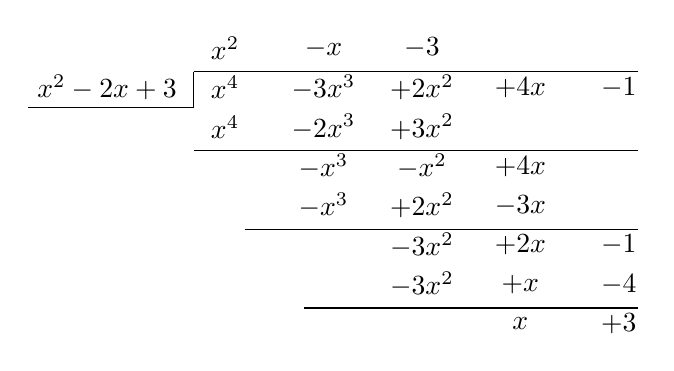
\begin{tikzpicture}[scale=0.5]
    \draw(-2, -1.5)--(2.2, -1.5);
    \draw(2.2, -1.5)--(2.2, -0.6);
    \draw(2.2, -0.6)--(13.5, -0.6);

    \node at(0, -1){$x^2-2x+3$};

    \node at(3, 0){$x^2$};
    \node at(5.5, 0){$-x$};
    \node at(8, 0){$-3$};

    \node at(3, -1){$x^4$};
    \node at(5.5, -1){$-3x^3$};
    \node at(8, -1){$+2x^2$};
    \node at(10.5, -1){$+4x$};
    \node at(13, -1){$-1$};

    \node at(3, -2){$x^4$};
    \node at(5.5, -2){$-2x^3$};
    \node at(8, -2){$+3x^2$};

    \draw(2.2, -2.6)--(13.5, -2.6);

    \node at(5.5, -3){$-x^3$};
    \node at(8, -3){$-x^2$};
    \node at(10.5, -3){$+4x$};

    \node at(5.5, -4){$-x^3$};
    \node at(8, -4){$+2x^2$};
    \node at(10.5, -4){$-3x$};

    \draw(3.5, -4.6)--(13.5, -4.6);

    \node at(8, -5){$-3x^2$};
    \node at(10.5, -5){$+2x$};
    \node at(13, -5){$-1$};

    \node at(8, -6){$-3x^2$};
    \node at(10.5, -6){$+x$};
    \node at(13, -6){$-4$};

    \draw(5, -6.6)--(13.5, -6.6);

    \node at(10.5, -7){$x$};
    \node at(13, -7){$+3$};

  \end{tikzpicture}
\end{figure}

\begin{definition}{因式分解定理}{}
元素$a\in F$是$f(x)\in F[x]$的零点当且仅当$x-a$是$F[x]$中的$f(x)$的因式.
\end{definition}

\begin{definition}{}{}
非零n次多项式$f(x)\in F[x]$在域F中最多有n个零点.
\end{definition}

\begin{definition}{}{}
非常数多项式$f(x)\in F[x]$在F上称为不可约\textnormal{(irreducible)}或$F[x]$上的不可约多项式\textnormal{(irreducible polynomial)},
如果f(x)不能表示为$F[x]$中的两个次数低于$f(x)$的多项式$g(x)$和$h(x)$的乘积$g(x)h(x)$.如果非常数多项式$f(x)\in F[x]$不是F上不可约的,则称$f(x)$为在F上可约的\textnormal{(reducible)}.
\end{definition}

\begin{definition}{}{}
设$f(x)\in F[x]$,且$f(x)$的次数为\textnormal{2}或\textnormal{3}.那么$f(x)$在F上是可约的当且仅当它在F中有一个零点.
\end{definition}

\begin{definition}{}{}
如果$f(x)\in \mathbb{Z}[x]$,则在$\mathbb{Q}[x]$中$f(x)$能分解为两个更低次数r和s的因式的乘积,当且仅当它在$\mathbb{Z}[x]$中具有相同次数r和s的因式分解.
\end{definition}

\begin{definition}{}{}
如果在$\mathbb{Z}[x]$中$f(x)=x^n+a_{n-1}xn^{n-1}+\cdots +a_0,a_0\neq 0$,且$f(x)$在$\mathbb{Q}$中有零点,则它在$\mathbb{Z}$中有零点m,且m比整除$a_0$.
\end{definition}

\begin{definition}{艾森斯坦准则}{}
设$p\in \mathbb{Z}为素数$.假设$f(x)=a_nx^n+\cdots +a_0$在$\mathbb{Z}[x]$中,
且$a\not \equiv 0\>(\textnormal{mod}\>p)$,
但对于所有$i<n$,$a_i\equiv 0\>(\textnormal{mod}\>p)$,
其中$a_0\not \equiv 0\>(\textnormal{mod}\>p^2)$,则f(x)在$\mathbb{Q}$上不可约.
\end{definition}

\section{$F[x]$中因式分解的唯一性}

\begin{definition}{}{}
如果F是一个域,那么每个非常数多项式$f(x)\in F[x]$都可以在$F[x]$中分解为不可约多项式的乘积,这些不可约多项式除了次序和F中的单位\textnormal{(也就是非零常数)}因子是唯一得到.
\end{definition}

\end{document}
